\documentclass[9pt,t]{beamer}
\usetheme{PastelGG}
\usepackage{tikz}
\usepackage{amsthm,amsmath,amsfonts,mathbbol,mathrsfs,stmaryrd,textcomp,hyperref}

%%-----------------------------------------------------------------------
%% Add a progress bar in footline
%% http://www.mrunix.de/forums/showpost.php?p=316577&postcount=3
%% ----------------------------------------------------------------------
\definecolor{lightgr}{rgb}{0.8235294117647058 0.615686274509804 0.6980392156862745}
\makeatletter
\addtobeamertemplate{footline}{%
  \color{lightgr}% to color the progressbar
  \hspace*{-\beamer@leftmargin}%
  \rule{\beamer@leftmargin}{2pt}%
  \rlap{\rule{\dimexpr
      \beamer@startpageofframe\dimexpr
      \beamer@rightmargin+\textwidth\relax/\beamer@endpageofdocument}{1pt}}
  % next 'empty' line is mandatory!

  \vspace{0\baselineskip}
  {}
}

\title{FRY: A Fast Approximation to ROAST Gene Set Test with Mean Aggregated Set Statistics}
\author[G\"{o}knur Giner]{G\"{o}knur Giner}
\date[November 1st, 2016]{November 1st, 2016,\\
AB$^3$ACBS Conference, Brisbane, AU}


\begin{document}

\begin{frame}[plain,t]
	\titlepage
\end{frame}

\section{Introduction}
% \begin{minipage}[pos][height][contentpos]{width} text \end{minipage} 
% pos: c(center), t(top), b(bottom) control the vertical alignment
% contentpos: c(center), t(top), b(bottom), s(spread)
% width: width of the box
\begin{frame}
	\frametitle{Gene Sets \textbf{\color{oxygenrose} (Pathways)}}
	\vspace{0.1cm}
\begin{minipage}[t][0.9\textheight][b]{0.6\textwidth}
\centering
\textbf{\color{oxygenpurple} BCL2 Family Genes}
\vspace{0.05cm}
\vfill
  \includegraphics[width=1\textwidth]{figures/bcl2}
  \vfill
\footnotesize \url{http://string-db.org}
\end{minipage}
\hspace{0.4cm}
\visible<2>{
\begin{minipage}[t][0.6\textheight][c]{0.3\textwidth}
\vspace{0.1cm}
\textbf{\color{oxygenpurple} Annotation Databases}
\vfill
  \includegraphics[width=1.2\textwidth]{figures/AnnotationDB}
\end{minipage}}
\end{frame}

\section{Pathway Analysis}
\begin{frame}
	\frametitle{Gene Set Tests  \textbf{\color{oxygenrose} (Pathway Analysis)}}
%	\only<1>{
%	\begin{minipage}[t]{0.5\textwidth}
%	\flushleft
%	{\color{oxygenpurple}\textbf{DNA Microarray}}
%	\includegraphics[width=0.7\textwidth]{figures/DNA_Microarray}
%	\end{minipage}
%	\hspace{0.2cm}
%	\visible<2>{
%	\begin{minipage}[t]{0.45\textwidth}
%	\flushleft
%	{\color{oxygenpurple}\textbf{RNA Sequencing}}
%	\includegraphics[width=0.9\textwidth]{figures/RNA_Sequencing}
%	\end{minipage}}}
%\only<2>{
\begin{columns}
	\column{0.6\textwidth}
	\textbf{\color{oxygenpurple} Differential expression analysis}
\begin{minipage}[c][1.1\textwidth][c]{\linewidth}
  	\centering
  \includegraphics[width=1\linewidth]{figures/de5_no_title}
\end{minipage}
	\column{0.4\textwidth}
	\visible<2-3>{
	\textbf{\color{oxygenpurple} Annotation Databases}
\begin{minipage}[t][0.4\textheight]{\linewidth}
\vspace{0.1cm}
  \includegraphics[width=0.6\linewidth]{figures/AnnotationDB}
\end{minipage}}
\visible<3>{
\textbf{\color{oxygenpurple} Type of Tests}
\begin{minipage}[t][0.5\textheight]{\linewidth}
 \textbf{\color{oxygenrose} Self-Contained$^*$} \\
  Tests the given pathway\\
 \\
 \textbf{\color{oxygenrose}Competitive$^*$}\\
 Ranks all of the pathways\\
 \\
\hfill $^*$\footnotesize Goeman \emph{et al.},  Bioinformatics (2007)
\end{minipage}}
\end{columns}	
%}
\end{frame}

\begin{frame}[c]
\frametitle{Existing Methods}
\begin{minipage}[t]{0.45\textwidth}
\flushleft
\textbf{\color{oxygenpurple}Over Representation Analysis (ORA)}
\vspace{0.1cm}
\begin{itemize}
\item Onto-Express(2001)
\item GeneMerge(2002)
\item DAVID(2003) 
\item GoMiner(2003)
\item FatiGO(2004)
\item GOstat(2004)
\end{itemize}
\end{minipage}
\hspace{0.4cm}
\begin{minipage}[t]{0.45\textwidth}
\flushleft
\textbf{\color{oxygenpurple}Functional Class Scoring (FCS)}
\vspace{0.1cm}
\begin{itemize}
\item GlobalTest(2004)
\item GSEA(2005)
\item sigPathway(2005)
\item SAFE(2005)
\item Category(2007)
\item SAM-GS(2007)
\item Roast(2010)
\item Camera(2012)
\end{itemize}
\end{minipage}
\vfill
\hfill $^*$\footnotesize Khatri \emph{et al.},  PLoS Comput Biol (2012)
\end{frame}

\begin{frame}[c]
\frametitle{Impact of Outdated Gene Annotations}
\textbf{\color{oxygenpurple}In 2015, $67\%$ of $3,900$ publications referenced outdated software that captured only $26\%$ of biological processes and pathways identified using current resources}
	 \centering
	 \vfill
	 \includegraphics[width=1\textwidth]{figures/tools}
	 \vfill
	 \hfill \footnotesize Wadi \emph{et al.},  Nature Methods (2016)
\end{frame}

\begin{frame}
	\frametitle{Assessment of Statistical Significance}
	\vspace{0.1cm}
	\begin{columns}
	\column{0.5\textwidth}	
	\centering
    \textbf{\color{oxygenpurple} Permutation Tests}
	\vbox to 0.5\textheight
	{
	\vspace{0.02\textwidth}
	%\vspace{0.1cm}
	\centering
    \includegraphics[width=0.7\textwidth]{figures/permutation}                
	\vspace{0.02cm}
	\begin{itemize}
		\item Require large number of samples 
		\item[]
		\item Applicable to limited type of experimental design
		\item[]
		\item GSEA is based on permutation test
		\end{itemize}
    }                       
	\column{0.5\textwidth}
	\centering
	{\color{oxygenpurple}\textbf{Rotation Tests}}
	\begin{itemize}
	\item Can produce unlimited number of rotated test statistics
	\item[]
	\item Applicable to complex arbitrary experimental designs
	\item[]	
	\item Roast: Rotation gene set tests for complex microarray experiments
	\end{itemize}
	\vspace{0.02cm}
	\includegraphics[width=0.6\textwidth]{figures/rotation}
	\end{columns}
\end{frame}

\section{Breast Cancer Example}
\begin{frame}
	\frametitle{Exploring Biological Processes in Breast Cancer}
	\centering
	\includegraphics[width=0.78\textwidth]{figures/breast_cancer_experiment}
\end{frame}

\begin{frame}
\frametitle{Barcode Plot}
\begin{minipage}[t][][b]{0.45\textwidth}	
	\begin{itemize}
		\item Both bi-directional
		\uncover<2-5>{\item[]
		\item Both applicable to arbitrary designs
		\item[]}
		\uncover<3-5>{
		\item Both work well with small sample sizes
		\item[]}
		\uncover<4-5>{
		\item Roast uses floor mean, mean50, mean square and mean to aggregate gene set level statistics
		\item[]}
		\uncover<5>{
		\item Fry uses only mean to aggregate gene level statistics}
	\end{itemize}
\end{minipage}
\begin{minipage}[t][][b]{0.54\textwidth}
	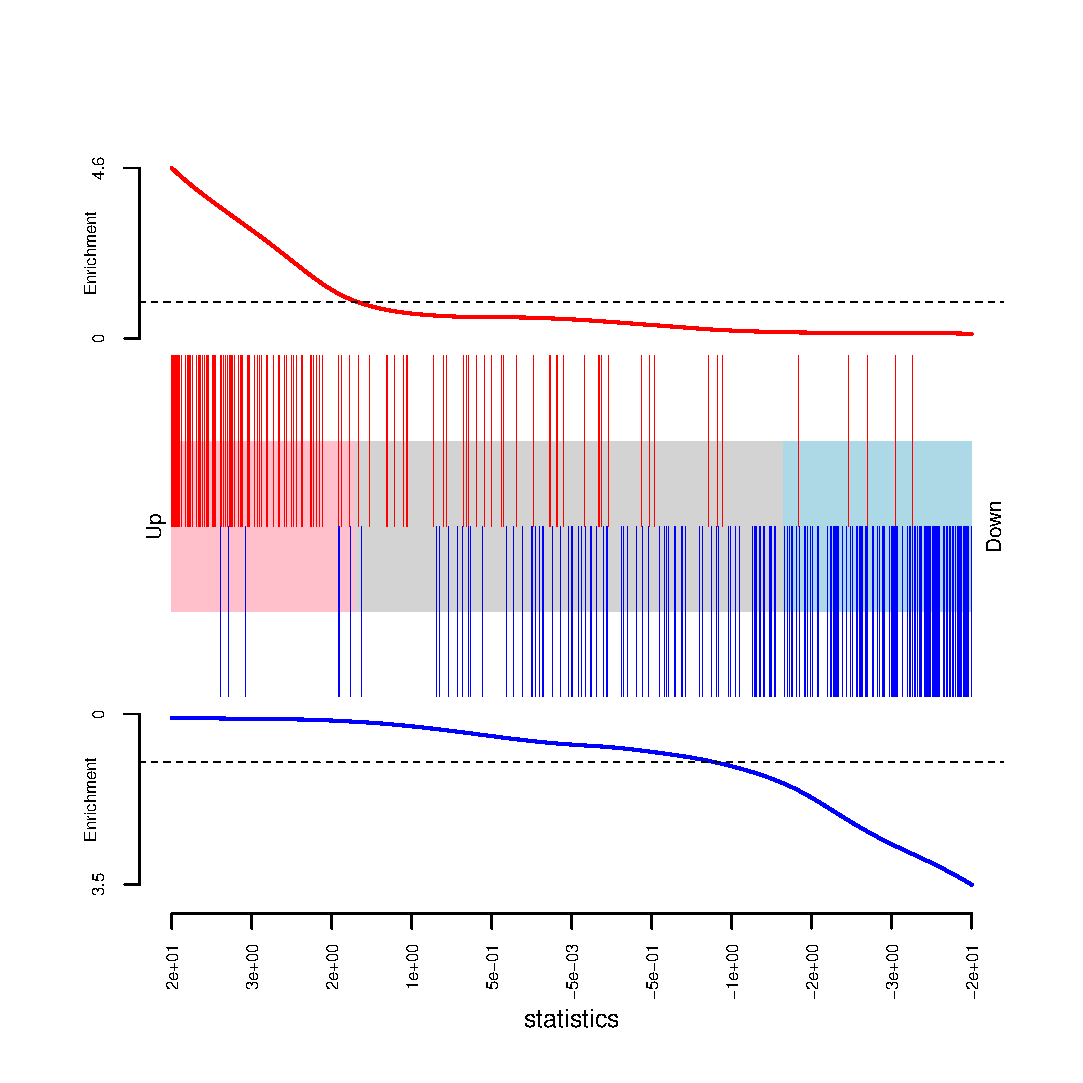
\includegraphics[width=1.1\textwidth]{figures/barcode_plot}
\end{minipage}
\end{frame}

\begin{frame}
\frametitle{Downsides of Roast}
Limitations when analysing large collections of sets\\
\vfill
 \uncover<2-4>{\textbf{\color{oxygenpurple} P-value resolution is limited by the number of rotations}}\\
\vfill
\uncover<3-4>{Top detected sets are all have the same p-values}\\
\vfill
\uncover<4>{P-values for each set may vary from run to run}\\
\vfill
\visible<2-4>{\begin{minipage}{1.4\textheight}
\includegraphics[width=1.1\textwidth]{figures/roast_table_short2}
\end{minipage}}
\end{frame}

\section{Why Fry}
\begin{frame}
\frametitle{Improved Features with Fry}
Assumes equal gene-wise variances\\
\vfill
 \uncover<2-5>{Gene level statistics are standardized using posterior gene variances} \\
\vfill
  \uncover<3-5>{\textbf{\color{oxygenpurple} Produces high-resolution exact p-values unlike roast}}\\
\vfill
\uncover<4-5>{Top detected sets are all have different p-values}\\
\vfill
\uncover<5>{P-values for each set does not vary from run to run}\\
\vfill
\visible<3-5>{\begin{minipage}{1.4\textheight}
\includegraphics[width=1.1\textwidth]{figures/fry_table_short2}
\end{minipage}}
\end{frame}

\begin{frame}
\frametitle{Fry is computationally very efficient}
\vfill
\large\textbf{\color{oxygenpurple}Over 4000 pathways are tested on an experiment with $15000+$ genes and $800+$ samples of TCGA Breast carcinoma simultaneously! Roast is rotated $10e5$ times!}\\
\vfill
\includegraphics[width=1\textwidth]{figures/speed}
\end{frame}

\begin{frame}
\frametitle{Fry outperforms Roast}
\begin{figure}
\includegraphics[width=1.2\textheight]{figures/power1}
\end{figure}
\end{frame}

\section{Fry Shiny Application}
\begin{frame}
\frametitle{Fry outperforms Roast}
\begin{figure}
\includegraphics[width=1.2\textheight]{figures/power1}
\end{figure}
\end{frame}
\section{Acknowledgement}
\begin{frame}[plain,t]
	\vspace{0.7cm}
	\textbf{\huge{Acknowledgements}}\\
	\vspace{1cm}
	
	\begin{minipage}[t]{0.49\textwidth}
	{\color{oxygenpurple}\textbf{WEHI Bioinformatics}}\\
	\vspace{0.20cm}
	
	\textbf{Gordon K. Smyth}\\
	Guido Pacini\\
	\vspace{0.35cm}
	
	{\color{oxygenpurple}\textbf{WEHI Population Health \\and Immunity}}\\
	\vspace{0.20cm}
	
	Saskia Freytag\\
	Roberto Bonelli\\
	\vspace{0.7cm}
	\end{minipage}%
	\begin{minipage}[t]{0.49\textwidth}
	{\color{oxygenpurple}\textbf{Data}}\\	
	{\color{oxygenrose}\textbf{Breast Cancer Laboratory Stem Cells and Cancer Division}}\\
	\vspace{0.20cm}
	
	Jane Visvader\\
	Delphine Merino\\
	Bhupinder Pal
	\vspace{0.75cm}
	
	
\includegraphics[width=1\textwidth]{WEHI}
	\vspace{1.35cm}
	
	
	\end{minipage}
\end{frame}

%\begin{frame}
%\url{http://shiny.bioinf.wehi.edu.au/giner.g/FRY_GeneSetExplorerApp/}{Fry_Shiny_App}
%\end{frame}
\end{document}

